\section{O Gás Ideal}

\epigraph{\justifying [...] eu era o mais disposto a contestar algumas Objeções
de \emph{Francisco Lineu}, uma vez que o medo de admitir o \emph{Vácuo} tem
prevalecido em tantas pessoas proeminentes criadas pela aclamada Filosofia das
Escolas, que mesmo que discordem com ele e entre si sobre a solução para o
\emph{Fenômeno} do Experimento de \emph{Torricelli}, concordam em atribui-la a
uma substância extremamente rarefeita que preenche o espaço deixado pelo
Mercúrio.}{\emph{Robert Boyle}, A Defence of the Doctrine Touching the Spring
and Weight of the Air (1662)}

\noindent Entre meados do século XVII houveram esforços dirigidos a entender a
natureza do ar, que até o final do século XIX tornaram-se um estudo da natureza
dos gases em geral de um ponto de vista termodinâmico. Com as limitações
experimentais e teóricas da época, foi desenvolvido o modelo mais simples
possível de um sistema termodinâmico com algum grau de liberdade além da própria
quantidade de calor absorvida, o \emph{gás ideal}. 

Dentro do escopo do que era possível experimentalmente, determinou-se que até
uma ótima precisão, o volume $V$, a \emph{pressão} $p$ - força por unidade de
área que uma amostra de gás exerce nas paredes de seu recipiente - e o número de
moléculas $N$ de uma amostra de gás caracterizam completamente sua isoterma, 
$$\frac{pV}{N}\equiv RT,$$
onde $T$ é uma escala de temperatura conhecida como \emph{temperatura
termodinâmica}, cujo valor numérico é determinado pela constante dos gases
ideais $R$, hoje fixada em $R=8{,}3145\,\mathrm{J/mol\,K}$, de forma que o ponto
triplo da água (ponto de coexistência entre seus três estados físicos) ocorre a
uma temperatura de $273{,}16\,\mathrm K$. A equação de estado acima normalmente
é escrita da forma
$$pV=NRT,$$
e recebe o nome de \emph{lei dos gases ideais}.

\subsection{Trabalho e Energia}

Uma descrição da termodinâmica de um sistema não se esgota com as equações de
estado. É necessário também um entendimento das maneiras que o sistema pode
realizar trabalho, e também identificar o comportamento da sua energia interna.
Para isso, considere uma pequena expansão do gás de um volume $V$ para $V+dV$.
Independente do formato do recipiente, podemos dividir sua superfície em
pequenas facetas $i$, cada uma com área $A_i$, deslocando-se perpendicularmente
por uma distância $dx_i$, contribuindo uma variação de volume $dV_i=A_idx_i$ de
forma que $\sum_idV_i=dV$.

\begin{figure}[H]
    \centering
    \begin{tikzpicture}
        \foreach \n in {1,...,3} {
            \path[name path global=v0\n,spath/save global=v0\n] 
                (\n,0) ..
                controls (\n+0.3,1.5) and (\n+0.3,2.5)
                .. (\n,4);
            \path[name path global=h0\n,spath/save global=h0\n] 
                (0,\n-0.1) ..
                controls (1.5,\n+0.3) and (2.5,\n+0.3)
                .. (4,\n-0.1);
            \path[name path global=v\n,spath/save global=v\n] 
                (\n+0.3,0.3) ..
                controls (\n+0.6,1.9) and (\n+0.5,2.7)
                .. (\n+0.3,4.3); 
            \path[name path global=h\n,spath/save global=h\n] 
                (0.3,\n+0.2) ..
                controls (1.7,\n+0.8) and (2.9,\n+0.7)
                .. (4.3,\n+0.2); 
        }
        \foreach \x/\y/\n in {3/3/0,3/2/1,2/2/2,2/3/3} {
            \path[name intersections={of={h0\x} and {v0\y},by={p\n}}];
            \path[name intersections={of={h\x} and {v\y},by={q\n}}];
        }
        \fill[lightgray] 
            \foreach \p/\q/\r in {
                h03/v0/reverse,
                v02/h0/reverse,
                h02/v0/,
                v03/h0/
            } {[
                spath/split at intersections with={\p}{\q2},
                spath/split at intersections with={\p}{\q3},
                spath/get components of={\p}\c,
                spath/use={\getComponentOf{\c}2,weld,\r},
            ]};
        \foreach \n in {1,...,3} {
            \draw[thick,darkgray,spath/use=v0\n];
            \draw[thick,darkgray,spath/use=h0\n];
            \draw[dashed,spath/use=v\n];
            \draw[dashed,spath/use=h\n];
        }
        \foreach \n in {1,...,3} 
            \draw[->,thick] 
                (p\n) -- (q\n);
        \draw[->,thick] 
            (p0) node[below left=-2] {$A_i$} 
            -- (q0) node[above right=-2] {$dx_i$};
    \end{tikzpicture}
\end{figure}

Supondo a pressão aproximadamente constante durante essa expansão, a força
atuando em cada uma dessas facetas é, por definição $F_i=pA_i$, e portanto sua
expansão realiza trabalho $\delta W_i=pA_idx_i=pdV_i$. Assim, ao longo da
superfície toda, o gás realiza um trabalho $\sum_i\delta W_i=pdV$. Concluimos
portanto que a expressão para o trabalho infinitesimal em termos de variáveis de
estado para o nosso gás deve ser
$$\delta W_\text{expansão}=-pdV,$$
ou seja, $V$ é a coordenada de trabalho conjugada ao coeficiente de trabalho
$-p$. Isso nos permite escrever que o trabalho realizado por um gás em um
processo traçado em um diagrama de pressão por volume é dado pela área sob a
curva em questão.

Por sua vez, a energia interna do gás ideal é tomada como proporcional a
quantidade e temperatura, dada por
$$U=\frac{NRT}{\gamma-1}.$$
O parâmetro $\gamma$ recebe o nome de \emph{coeficiente de Poisson}, e para
gases nobres como hélio e neônio temos $\gamma=5/3$, enquanto para gases
diatômicos usuais como oxigênio e nitrogênio temos $\gamma=7/5$. 

\subsection{Processos Importantes}

Aqui vamos encontrar expressões para o trabalho realizado pelo gás e a
capacidade térmica de alguns processos de maior incidência e importância
teórica, assim como traçá-los em um diagrama de pressão por volume.

\subsubsection{Isocórico}

O processo isocórico é o processo contínuo em que mantemos as coordenadas de
trabalho (volume) constantes.
\begin{figure}[H]
    \centering
    \begin{tikzpicture}
        \draw [->, thick]
            (0,0) -- (5,0) node[below] {$V$};
        \draw [->, thick]
            (0,0) -- (0,4) node[left] {$p$};
        \draw
            (2.5,0.2) -- (2.5,-0.2) node[below] {$V_0$};
        \draw
            (0.2,1.2) -- (-0.2,1.2) node[left] {$p_i$};
        \draw
            (0.2,2.8) -- (-0.2,2.8) node[left] {$p_f$};
        \draw[ultra thick,postaction={mid arrow}]
            (2.5,1.2) -- (2.5,2.8);
        \fill
            (2.5,1.2) circle (0.05);
        \fill
            (2.5,2.8) circle (0.05);
    \end{tikzpicture}
\end{figure}
A cada passo vale que $dV=0$, e portanto o trabalho deste processo é $$W_\text{
isocórico}=0.$$ A capacidade térmica, por sua vez é
$$C_V=\frac{\delta Q}{dT}=\frac{dU+pdV}{dT}=\frac{NR}{\gamma-1}.$$

\subsubsection{Isobárico}

O processo isobárico é o processo contínuo em que mantemos os coeficientes de
trabalho (pressão) constantes.
\begin{figure}[H]
    \centering
    \begin{tikzpicture}
        \draw[->, thick] 
            (0,0) -- (5,0) node[below] {$V$};
        \draw[->, thick]
            (0,0) -- (0,4) node[left] {$p$};
        \draw 
            (1.5,0.2) -- (1.5,-0.2) node[below] {$V_i$};
        \draw
            (3.5,0.2) -- (3.5,-0.2) node[below] {$V_f$};
        \draw
            (0.2,2) -- (-0.2,2) node[left] {$p_0$};
        \draw[ultra thick,postaction={mid arrow}]
            (1.5,2) -- (3.5,2);
        \fill
            (1.5,2) circle (0.05);
        \fill
            (3.5,2) circle (0.05);
    \end{tikzpicture}
\end{figure}
A pressão no processo todo é constante, e portanto a integral do trabalho é
simplesmente
$$W_\text{isobárico}=\int_{V_i}^{V_f}p\,dV=p_0(V_f-V_i).$$
A capacidade térmica torna-se
$$C_p=\frac{\delta Q}{dT}=\frac{dU+pdV}{dT}=\frac{\gamma NR}{\gamma-1}
=\gamma C_V = C_V+NR.$$

\subsubsection{Isotérmico}

O processo isotérmico é o processo contínuo em que mantemos a temperatura
constante. Para o gás ideal isso significa simplesmente que $pV=\text{const.}$
\begin{figure}[H]
    \centering
    \begin{tikzpicture}
        \draw[->, thick]
            (0,0) -- (5,0) node[below] {$V$};
        \draw[->, thick]
            (0,0) -- (0,4) node[left] {$p$};
        \draw
            (1.5,0.2) -- (1.5,-0.2) node[below] {$V_i$};
        \draw
            (3.5,0.2) -- (3.5,-0.2) node[below] {$V_f$};
        \draw
            (0.2,1.2) -- (-0.2,1.2) node[left] {$p_f$};
        \draw
            (0.2,2.8) -- (-0.2,2.8) node[left] {$p_i$};
        \draw[ultra thick,postaction={mid arrow},samples=10,domain=1.5:3.5]
            plot (\x,{4.2/\x});
        \fill
            (1.5,2.8) circle (0.05);
        \fill
            (3.5,1.2) circle (0.05);
    \end{tikzpicture}
\end{figure}
A expressão para o trabalho fica mais simétrica quando expressada em termos da
temperatura de operação $T_0$:
$$W_\text{isotérmico}=\int_{V_i}^{V_f}p\,dV=NRT_0\int_{V_i}^{V_f}\frac{1}{V}
\,dV= NRT_0\log\frac{V_f}{V_i}=NRT_0\log\frac{p_i}{p_f}.$$
Como não há variação de temperatura, a capacidade térmica diverge.

\subsubsection{Isotérmico}

O processo adiabático é o processo contínuo em que mantemos o sistema isolado,
sem perimitir trocas de calor.
\begin{figure}[H]
    \centering
    \begin{tikzpicture}
        \draw[->, thick]
            (0,0) -- (5,0) node[below] {$V$};
        \draw[->, thick]
            (0,0) -- (0,4) node[left] {$p$};
        \draw
            (1.5,0.2) -- (1.5,-0.2) node[below] {$V_i$};
        \draw
            (3.5,0.2) -- (3.5,-0.2) node[below] {$V_f$};
        \draw
            (0.2,0.83) -- (-0.2,0.83) node[left] {$p_f$};
        \draw
            (0.2,3.4) -- (-0.2,3.4) node[left] {$p_i$};
        \draw[ultra thick,postaction={mid arrow},samples=10,domain=1.5:3.5]
            plot (\x,{3.4*(1.5/\x)^(5/3)});
        \fill
            (1.5,3.4) circle (0.05);
        \fill
            (3.5,0.83) circle (0.05);
    \end{tikzpicture}
\end{figure}
Partindo da primeira lei $dU+pdV=0$ e da equação de estado $pV=NRT$ podemos
deduzir três relações que se realizam no processo adiabático:
\begin{align*}
    \frac{dp}{p}+\gamma\frac{dV}{V}=0&\Leftrightarrow pV^\gamma=\text{const.}\\
    \frac{dT}{T}+(\gamma-1)\frac{dV}{V}=0&\Leftrightarrow TV^{\gamma-1}=
    \text{const.}\\
    \gamma\frac{dT}{T}-(\gamma-1)\frac{dp}{p}=
    0&\Leftrightarrow T^\gamma/p^{\gamma-1}=\text{const.}\\
\end{align*}
Note que no diagrama acima com $\gamma=5/3$ a curva é mais inclinada do que a
isoterma do diagrama anterior. Como não há troca de calor, podemos calcular o
trabalho realizado diretamente pela variação de energia interna,
$$W_\text{adiabático}=U_i-U_f=\frac{NR(T_f-T_i)}{\gamma-1}
=\frac{p_iV_i-p_fV_f}{\gamma-1}.$$
Como não há calor absorvido, a capacidade térmica é zero.

\subsection{Problemas}

\begin{enumerate}
    \item
        A lei de Stevin relaciona a variação de pressão $p$ de um fluido de
        densidade $\rho$ sob ação da gravidade $g$ com a variação de altura
        $h$ como
        $$dp=-\rho gdh.$$
        \begin{enumerate}
            \item 
                Considere o fluido como sendo um gás ideal de massa molar
                $\mu$. Encontre a densidade $\rho$ como função da pressão $p$ e
                da temperatura $T$.
                \answer{$\rho=\frac{\mu p}{RT}$}
            \item
                Partindo da Lei de Stevin, escreva uma equação para como a
                pressão varia com a altura.
                \answer{$\frac{dp}{dh}=-\frac{\mu g}{RT}p$}
            \item 
                Seja $p_0$ a pressão atmosférica no nível do mar, marcado como
                $h=0$. Supondo que a temperatura da atmosfera seja constante com
                a altura, encontre $p(h)$.
                \answer{$p=p_0e^{-\mu gh/RT}$}
            \item 
                O monte Everest possui uma altura de $8848\,\mathrm{m}$ com
                relação ao nível do mar. Suponha que a temperatura do ar é
                constante $T=273\,\mathrm{K}$ e a gravidade $g=9{,}79
                \,\mathrm{m/s^2}$. Dado que a pressão no topo do everest é
                $0{,}333p_0$, estime a massa molar $\mu$ do ar atmosférico.
                \answer{
                    $\mu=\frac{RT}{gh}\log\left(\frac{p_0}{p}\right)=28.8
                    \,\mathrm{g/mol}$
                }
            \item 
                Por fim, supondo que o ar seja composto de gás nitrogênio 
                $\mathrm{N_2}$ e oxigênio $\mathrm{O_2}$, encontre a proporção
                $x$ de oxigênio na atmosfera.
                \answer{
                    $x=\frac{\mu-\mu_\mathrm{N_2}}
                    {\mu_\mathrm{O_2}-\mu_\mathrm{N_2}}=20\%$
                }
        \end{enumerate}

    \item
        (SOIF 2001) Um cilíndro cheio de gás tem a área da seção reta igual a
        $A=10\,\mathrm{cm^2}$ e é fechado por um êmbolo pesado e móvel. O
        cilíndro começa a subir com aceleração de $a=20\,\mathrm{m/s^2}$ e,
        mantendo a temperatura do gás constante, seu volume fica $\eta=2/3$ do
        original. Ache a massa $M$ do êmbolo sabendo que a gravidade local é $g=
        10\,\mathrm{m/s^2}$ e a pressão atmosférica é $p_0=10^5
        \,\mathrm{N/m^2}$. 
        \answer{$M=\frac{(1-\eta)p_0A}{\eta a-(1-\eta)g}=3{,}3\,\mathrm{kg}$}

    \item
        (Irodov) Defina a taxa de evacuação $r$ de um gás como o volume perdido
        por unidade de tempo quando medido à própria pressão e temperatura do
        gás. Encontre a pressão $p$ como função do tempo $t$ para um gás dentro
        de um recipiente de volume $V$ que expulsa gás a uma taxa de evacuação
        constante $r$. Suponha que a temperatura do gás não muda durante o
        processo e que a pressão inicial é $p_0$.
        \answer{$p=p_0e^{-rt/V}$}

    \item
        Considere um cilíndro vertical fechado em baixo e tampado por um pistão
        móvel de massa $M$. Dentro do cilíndro há uma massa $m$ de gás ideal de
        massa molar $\mu$. Sendo $g$ a aceleração da gravidade e supondo que
        fora do cilíndro há vácuo, encontre a altura $H$ do pistão móvel como
        função da temperatura $T$ do gás.
        \answer{$H=\frac{RT}{\mu g}\log\left(1+\frac{m}{M}\right)$}

    \item
        (SOIF 2005) Um cilíndro com paredes termicamente isoladas contém duas
        espécies de gás distintas, separadas por uma parede isolante. O primeiro
        gás tem coeficiente de Poisson $\gamma_1$, pressão $p_1$, volume $V_1$ e
        temperatura $T_1$. O segundo tem respectivos $\gamma_2,p_2,V_2$ e $T_2$.
        Como fica a pressão $p$ e temperatura $T$ no cilíndro após retirarmos a
        parede interna e esperarmos o equilíbrio termodinâmico?
        \answer{
            $T=\frac{\frac{p_1V_1}{\gamma_1-1}+\frac{p_2V_2}{\gamma_2-1}}
            {\frac{p_1V_1}{T_1(\gamma_1-1)}+\frac{p_2V_2}{T_2(\gamma_2-1)}},
            \quad p=\frac{\frac{p_1V_1}{T_1}+\frac{p_2V_2}{T_2}}{V_1+V_2}T$
        }

    \item
        Um tubo vertical liso possui dois raios, com a área superior maior do
        que a inferior por uma parcela $A$, equipado com um par de pistões de
        massa total $M$, como na figura abaixo.
        \begin{figure}[H]
            \centering
            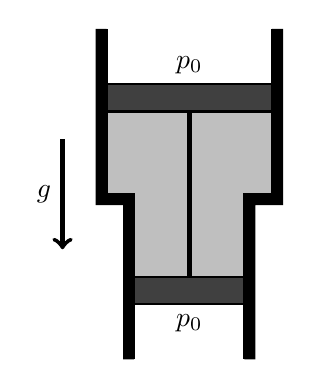
\begin{tikzpicture}[scale=0.7]
                \fill[lightgray]
                    (1.5,1.5) -- (-1.5,1.5) -- (-1.5,0) -- (-1,0)
                    -- (-1,-1.5) -- (1,-1.5) -- (1,0) -- (1.5,0) -- (1.5,1.5);
                \fill[darkgray]
                    (-1.5,2) -- (1.5,2) -- (1.5,1.5) -- (-1.5,1.5);
                \draw[thick]
                    (-1.5,2) -- node[pos=0.5,above] {$p_0$} (1.5,2)
                    -- (1.5,1.5) -- (-1.5,1.5) -- (-1.5,2);
                \fill[darkgray]
                    (-1,-2) -- (1,-2) -- (1,-1.5) -- (-1,-1.5);
                \draw[thick]
                    (-1,-2) -- node[pos=0.5,below] {$p_0$} (1,-2)
                    -- (1,-1.5) -- (-1,-1.5) -- (-1,-2);
                \fill
                    (-1.5,3) -- (-1.5,0) -- (-1,0) -- (-1,-3) -- (-1.2,-3)
                    -- (-1.2,-0.2) -- (-1.7,-0.2) -- (-1.7,3);
                \draw[thick]
                    (-1.5,3) -- (-1.5,0) -- (-1,0) -- (-1,-3);
                \draw[thick]
                    (1.5,3) -- (1.5,0) -- (1,0) -- (1,-3);
                \fill
                    (1.5,3) -- (1.5,0) -- (1,0) -- (1,-3) -- (1.2,-3)
                    -- (1.2,-0.2) -- (1.7,-0.2) -- (1.7,3);
                \draw[ultra thick]
                    (0,1.5) -- (0,-1.5);
                \draw[ultra thick,->]
                    (-2.3,1) -- node[pos=0.5,left] {$g$} (-2.3,-1);
            \end{tikzpicture}
        \end{figure}
        Cada pistão move-se na seção correspondente, e o menor possui massa $m$
        e área $a$. Uma quantidade $N$ de gás ideal de massa desprezível
        encontra-se entre os pistões, e estes estão presos um ao outro por um
        fio inextensível de comprimento $L$. A pressão externa aos tubos é $p_0$
        e a gravidade local é $g$. Inicialmente, a temperatura do gás é baixa,
        de forma que o pistão superior está apoiado na junção das duas seções, e
        o fio encontra-se frouxo.
        \begin{enumerate}
            \item
                Encontre a temperatura $T_0$ a partir da qual o fio fica
                tensionado
                \answer{$T_0=\frac{(p_0a-mg)L}{NR}$}
            \item
                Encontre a temperatura $T_1$ a partir da qual o pistão superior
                começa a subir. Esta é maior ou menor do que $T_0$?
                \answer{$T_1=\frac {(p_0A+Mg)L}{NR}>T_0$}
            \item
                Encontre a temperatura máxima $T_\text{máx}$ a partir da qual o
                pistão de baixo descarrilha de sua seção e o gás vaza para o
                meio externo
                \answer{$T_\text{máx}=T_1\left(1+\frac{a}{A}\right)$}
            \item
                Faça um gráfico da pressão $p$ como função da temperatura para
                este sistema
                \answer{
                    \begin{tikzpicture}
                        \draw[very thick,->]
                            (0,0) -- (3,0) node[below] {$T$};
                        \draw[very thick,->]
                            (0,0) -- (0,2) node[above] {$p$};
                        \draw[ultra thick]
                            (0,0.6) -- (0.4,0.6) -- (1.3,1.5) -- (2.3,1.5);
                        \filldraw[fill=white]
                            (2.3,1.5) circle (0.05);
                        \draw
                            (0.1,0.6) -- (-0.1,0.6) node[left] {$p_0-mg/a$};
                        \draw
                            (0.1,1.5) -- (-0.1,1.5) node[left] {$p_0+Mg/A$};
                        \draw
                            (0.4,0.1) -- (0.4,-0.1) node[below] {$T_0$};
                        \draw
                            (1.3,0.1) -- (1.3,-0.1) node[below] {$T_1$};
                        \draw
                            (2.3,0.1) -- (2.3,-0.1) node[below] 
                            {$T_\text{máx}$};
                    \end{tikzpicture}
                }
        \end{enumerate}

    \item
        Mostre que a para um processo num gás ideal
        $$pV^\alpha=\text{const}\Leftrightarrow C=\text{const}.$$
        encontrando uma relação entre $C$ e $\alpha$ para $N$ mols de um gás
        ideal de coeficiente de Poisson $\gamma$
        \answer{$C=NR\left(\frac{1}{\gamma-1}-\frac{1}{\alpha-1}\right)$}

    \item
        (Irodov) Certa quantidade de gás ideal de coeficiente de Poisson
        $\gamma$ realiza um processo em que sua capacidade térmica é função da
        temperatura dada por $C=p_0V_0/T$. Encontre uma relação entre a pressão
        e o volume do gás nesse processo, sabendo que ele passa pelo ponto
        $(p_0,V_0,T_0)$.
        \answer{$pV^\gamma=p_0V_0^\gamma e^{\left(1-\frac{p_0V_0}{pV}\right)}$}

    \item
        Um recipiente isolado termicamente é dividido por um pistão que pode
        movimentar-se sem atrito, conforme a figura abaixo.
        \begin{figure}[H]
            \centering
            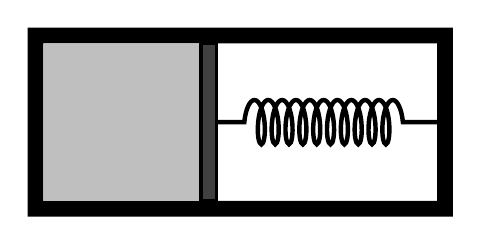
\begin{tikzpicture}
                \fill 
                    (0,0) -- (5,0) -- (5,2) -- (0,2) -- (0,0)
                    -- (-0.2,-0.2) -- (-0.2,2.2) -- (5.2,2.2)
                    -- (5.2,-0.2) -- (-0.2,-0.2) -- (0,0);
                \fill[lightgray]
                    (0,0) -- (2,0) -- (2,2) -- (0,2) -- (0,0);
                \fill[darkgray]
                    (2,0) -- (2,2) -- (2.2,2) -- (2.2,0) -- (2,0);
                \draw[very thick]
                    (2,0) -- (2,2) -- (2.2,2) -- (2.2,0) -- (2,0);
                \draw[decoration={
                    coil,
                    segment length=5,
                    aspect=0.3,
                    amplitude=8,
                    pre length=10,
                    post length=10
                },decorate,ultra thick]
                    (2.2,1) -- (5,1);
            \end{tikzpicture}
        \end{figure}
        A parte da esquerda é preenchida com um mol de gás ideal monoatômico, e
        a parte da direita encontra-se evacuada. O pistão é conectado à parede
        da direita por meio de uma mola cujo comprimento livre é igual ao
        comprimento total do recipiente. Determine o calor especifico molar $c$
        do gás sob essas condições em função da constante dos gases ideais $R$.
        \answer{$c=2R$}

    \item
        Um gás ideal de coeficiente de Poission $\gamma$ com $N$ moléculas é
        sujeito aos seguintes processos:
        \begin{enumerate}
            \item
                $p=p_0(1-V/V_0)$
                \answer{
                    $T=\frac{T_0}{4},\,c=R\left(\frac{1}{\gamma-1}+
                    \frac{V_0-V}{V_0-2V}\right)$
                }
            \item
                $p=p_0(1-(V/V_0)^2)$
                \answer{
                    $T=\frac{2T_0}{3\sqrt3},\,c=R\left(\frac{1}{\gamma-1}+
                    \frac{V_0^2-V^2}{V_0^2-3V^2}\right)$
                }
            \item
                $p=p_0e^{-V/V_0}$
                \answer{
                    $T=\frac{T_0}{e},\,c=R\left(\frac{1}{\gamma-1}+
                    \frac{V_0}{V_0-V}\right)$
                }
        \end{enumerate}
        Onde $p_0$ e $V_0$ são constantes positivas. Encontre a temperatura
        máxima em termos de $T_0=\frac{p_0V_0}{NR}$ e o calor específico molar
        como função do volume $V$ e das constantes $\gamma$, $R$, e $V_0$.

    \item
        (SOIF 2004) Considere um cilíndro hermeticamente vedado com paredes
        adiabáticas, fechado em ambas as extremidades e dividido em duas partes
        por um êmbolo isolante que pode mover-se livremente sem atrito.
        Inicialmente o volume, pressão e temperatura de gases em cada parte do
        cilíndro é $V_0,p_0$ e $T_0$, respectivamente. No lado direito do
        cilíndro é colocado um aquecedor que aquece o gás até que sua pressão
        atinja $\alpha p_0$. Considerando os gases ideais de coeficiente de
        Poisson $\gamma$, encontre
        \begin{enumerate}
            \item
                O volume final do lado esquerdo
                \answer{$V_L=V_0\alpha^{-\frac{1}{\gamma}}$}
            \item
                a temperatura final do lado esquerdo
                \answer{$T_L=T_0\alpha^{1-\frac{1}{\gamma}}$}
            \item
                a temperatura final do lado direito
                \answer{
                    $T_R=T_0\alpha\left(2-\alpha^{-\frac{1}{\gamma}}\right)$
                }
            \item
                o trabalho efetuado sobre o gás do lado esquerdo
                \answer{$W=p_0V_0\left(\alpha^{1-\frac{1}{\gamma}}-1\right)$}
        \end{enumerate}

    \item
        Considere um longo cilíndro horizontal semiaberto. Coloque-o para girar,
        com seu eixo na vertical posicionado no lado aberto, a uma velocidade
        angular $\omega$. Encontre a pressão $p$ do ar dentro do tubo como
        função da distância $r$ do eixo de rotação. Suponha o ar um gás ideal de
        temperatura $T$ e massa molar $\mu$, e que a pressão atmosférica é $p_0$.
        \answer{$p=p_0e^\frac{\mu\omega^2r^2}{2RT}$}

    \item
        Um recipiente contém $N$ móls de hélio. Este gás passa por um processo
        termodinâmico em que sua capacidade térmica depende da temperatura como
        $C=\frac{3NRT}{4T_0}$, sendo $T_0$ a temperatura inicial do gás.
        Encontre o trabalho realizado sobre o gás ao longo deste processo até
        que ele seja comprimido ao seu volume mínimo.
        \answer{$W=\frac{3}{8}NRT_0$}

    \item
        (IPhO 1996) Considere duas bolas metálicas idênticas. Uma está pendurada
        no teto pela superfície enquanto a outra está apoiada no chão, como na
        figura abaixo.
        \begin{figure}[H]
            \centering
            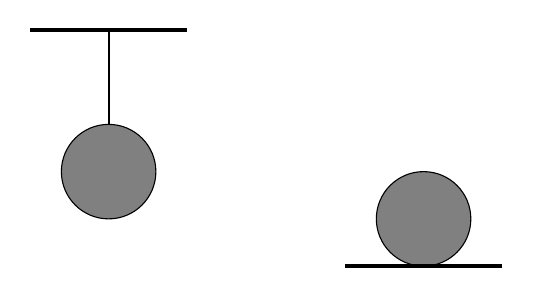
\begin{tikzpicture}
                \draw[thick]
                    (-2,2) -- (-2,0.8);
                \filldraw[fill=gray]
                    (-2,0.2) circle (0.6);
                \draw[ultra thick]
                    (-3,2) -- (-1,2);
                \filldraw[fill=gray]
                    (2,-0.4) circle (0.6);
                \draw[ultra thick]
                    (3,-1) -- (1,-1);
            \end{tikzpicture}
        \end{figure}
        Uma mesma pequena quantidade de calor é fornecida para ambas as bolas.
        Qual delas fica com uma temperatura maior?
        \answer{a bolinha pendurada}

    \item
        Considere um recipiente com paredes isolantes e rígidas inicialmente
        evacuado. Faz-se um pequeno furo no recipiente e ar atmosférico entra
        lentamente. Encontre a temperatura do ar no interior do balão no momento
        em que o fluxo de ar para dentro cessa. O ar atmosférico pode ser
        considerado um gás ideal de coeficiente de Poisson $\gamma$ e
        temperatura $T_0$.
        \answer{$T=\gamma T_0$}

    \item
        O método de Rüchhardt para medir o coeficiente de Poisson do ar consiste
        no seguinte. Uma garrafa de volume $V_0$ é preenchida com ar
        atmosférico. Seu gargalo tem área $A$ e neste é colocado uma bola justa
        de massa $m$, solta a partir do repouso. Dado que a gravidade local é
        $g$ e a pressão atmosférica é $p_0$.
        \begin{figure}[H]
            \centering
            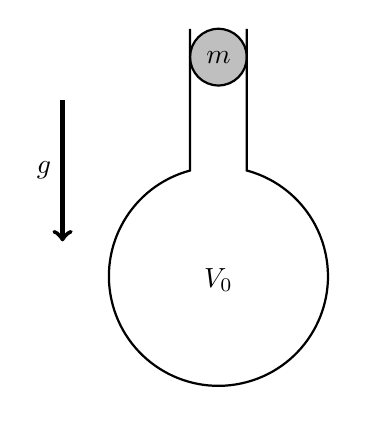
\begin{tikzpicture}[scale=1.8]
                \fill[lightgray]
                    (0,0.8) circle (0.2);
                \draw[thick]
                    (0,0.8) node {$m$} circle (0.2);
                \draw[thick]
                    (-0.2,1) -- (-0.2, 0) 
                    arc (105:435:{0.2/sin(15)}) -- (0.2,1);
                \draw
                    (0,{-0.2/sin(15)}) node {$V_0$};
                \draw[ultra thick,->]
                    (-1.1,0.5) -- node[pos=0.5,left] {$g$} (-1.1,-0.5);
            \end{tikzpicture}
        \end{figure}

        Desprezando atritos e trocas de calor entre a garrafa e o meio externo e
        supondo que o volume do gargalo é muito menor do que o do resto da
        garrafa, encontre
        \begin{enumerate}
            \item
                A distância máxima $L$ que a bola afunda no gargalo após ser
                solta
                \answer{$L=\frac{2mgV_0}{\gamma A^2p_0}$}
            \item
                O período $\tau$ do movimento subsequente
                \answer{$\tau=\frac{2\pi}{A}\sqrt\frac{mV_0}{\gamma p_0}$}
        \end{enumerate}
        Pode ser útil que
        $$|nx|\ll1\Rightarrow(1+x)^n\approx1+nx.$$

    \item
        (200 PPP) Considere um cilíndro isolado fechado que possui uma parede
        condutora móvel em seu interior que separa duas quantidades iguais de
        gás ideal de coeficiente de Poisson $\gamma$. Se aplicarmos uma força 
        externa constante muito grande nesta parede e esperarmos o equilíbrio
        térmico, como ficará a razão entre os volumes das partes expandidas e
        contraidas? 
        \answer{$r=\frac{\sqrt\gamma+1}{\sqrt\gamma-1}$}

    \item
        Um cilíndro vertical isolante possui a base fechada e dois pistões de
        peso desprezível. Entre a base e o primeiro pistão, diatérmico, existe
        certa quantidade de hélio. Entre o primeiro e o segundo pistão,
        isolante, existe certa quantidade de hidrogênio. Inicialmente, o volume
        de hidrogênio é 1/3 do volume de hélio. Dá se uma quantidade de calor
        $Q$ para o hélio e o pistão superior move-se para cima uma distância
        $D$. Após certo tempo, há outra movimentação do pistão superior. Quanto
        ele se moveu e para qual direção?
        \answer{cai de $D/7$}

    \item
        Um fino tubo circular de raio $r$ é disposto como na figura abaixo.
        \begin{figure}[H]
            \centering
            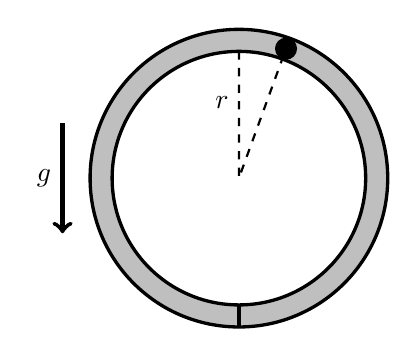
\begin{tikzpicture}[scale=0.7]
                \fill[lightgray,even odd rule]
                    (0,0) circle (2.3) (0,0) circle (2.7);
                \draw[very thick]
                    (0,0) circle (2.3);
                \draw[very thick]
                    (0,0) circle (2.7);
                \draw[ultra thick]
                    (0,-2.7) -- (0,-2.3);
                \fill
                    ({2.5*sin(20)},{2.5*cos(20)}) circle (0.2);
                \draw[thick,dashed]
                    (0,2.3) -- node[pos=0.4,left] {$r$} 
                    (0,0) -- ({2.3*sin(20)},{2.3*cos(20)});
                \draw[ultra thick,->]
                    (-3.2,1) -- node[pos=0.5,left] {$g$} (-3.2,-1);
            \end{tikzpicture}
        \end{figure}
        Na parte inferior do tubo há uma parede, e dentro dele há uma bolinha de
        massa $m$ que pode se deslocar sem atrito ao longo do tubo, separando-o
        em duas partes ambas contendo uma quantidade $N$ de gás ideal. Quando a
        temperatura do sistema é alta, a bolinha tende a ficar equilibrada no
        ápice do tubo. No entanto quando a temperatura cai abaixo de certo valor
        $T_c$, este equilíbrio mecânico torna-se instável e a bolinha cai para
        algum dos lados e encontra um novo ponto de equilíbrio.
        \begin{enumerate}
            \item
                Encontre a temperatura crítica $T_c$
                \answer{$T_c=\frac{\pi^2mgr}{2NR}$}
            \item
                A capacidade térmica do sistema é descontínua em $T_c$. Encontre
                a diferença de capacidade térmica $\Delta C$ entre temperaturas
                um pouco menores que $T_c$ e um pouco maiores que $T_c$. 
                \answer{$\Delta C=\frac{NR}{1+\pi^2/6}$}
        \end{enumerate}
        Pode ser útil que
        $$|x|\ll1\Rightarrow\sin x\approx x-\frac{1}{6}x^3.$$
\end{enumerate}
